\documentclass{beamer}

\usepackage{tikz}
\usepackage{graphicx}
\usepackage{caption}

\begin{document}
\captionsetup{font=scriptsize, labelfont=scriptsize}
\setbeamertemplate{caption}{\raggedright\insertcaption\par}

\title{Frequent-Collision Blockchains for Local Geographic Authentication}
\author{Ryan Robinett and Tiago Royer}
\date{10 Dec 2019}
\institute[CMSC33300]{
    CMSC33300 --- Networks \\
    Department of Computer Science \\
    University of Chicago
}

\begin{frame}
    \titlepage
\end{frame}

\begin{frame}
	\frametitle{Problem motivation}

	\begin{itemize}
		\item Geographic Authentication:
			proving you are/were in a certain location
			at a certain point in time
		\item Goal: decentralized, historic geographic authentication
			\begin{itemize}
				\item Conventional geographic authentication asks, \textbf{``Where are you now?''}
				\item We want to ask, \textbf{``Where have you been in the recent past?''}
			\end{itemize}
		\item Proposed Solution:
			\begin{itemize}
				\item Peer-to-peer ``checkins'' over a \textbf{smartphone
					\textit{ad hoc} network (SPAN)}
				\item Store checkins using a \textbf{blockchain}
				\item \textbf{Forking}: want to use this as a feature,
					rather than a bug
			\end{itemize}
	\end{itemize}
\end{frame}

\begin{frame}
	\frametitle{Blockchains and Forking}

	\begin{columns}{}
		\begin{column}{0.5\textwidth}
			\begin{figure}
				\centering
				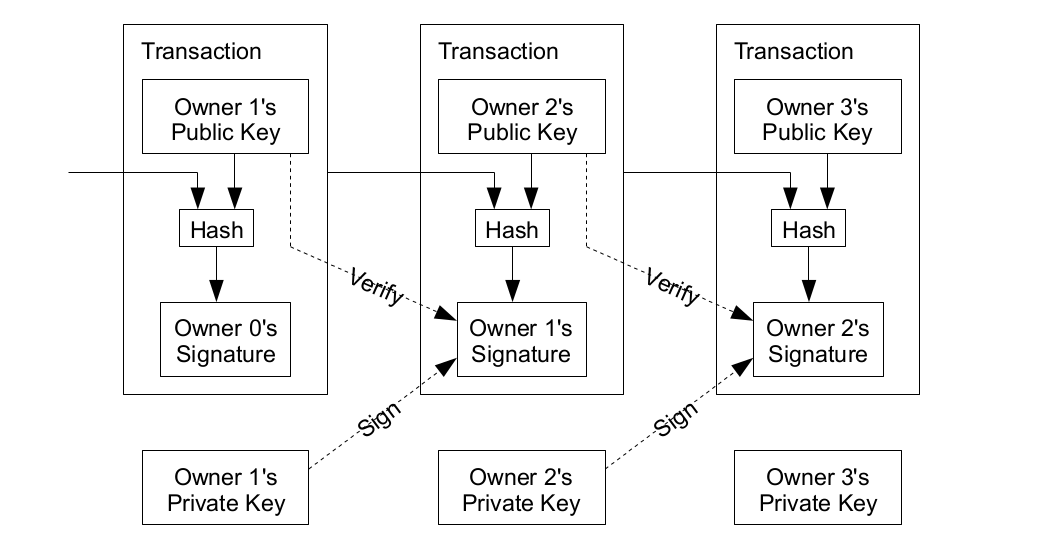
\includegraphics[width=\textwidth]{nakamoto_hashes.png}
				\caption{Nakamoto 2008}
			\end{figure}

			\begin{figure}
				\centering
				\vspace{-1cm}
				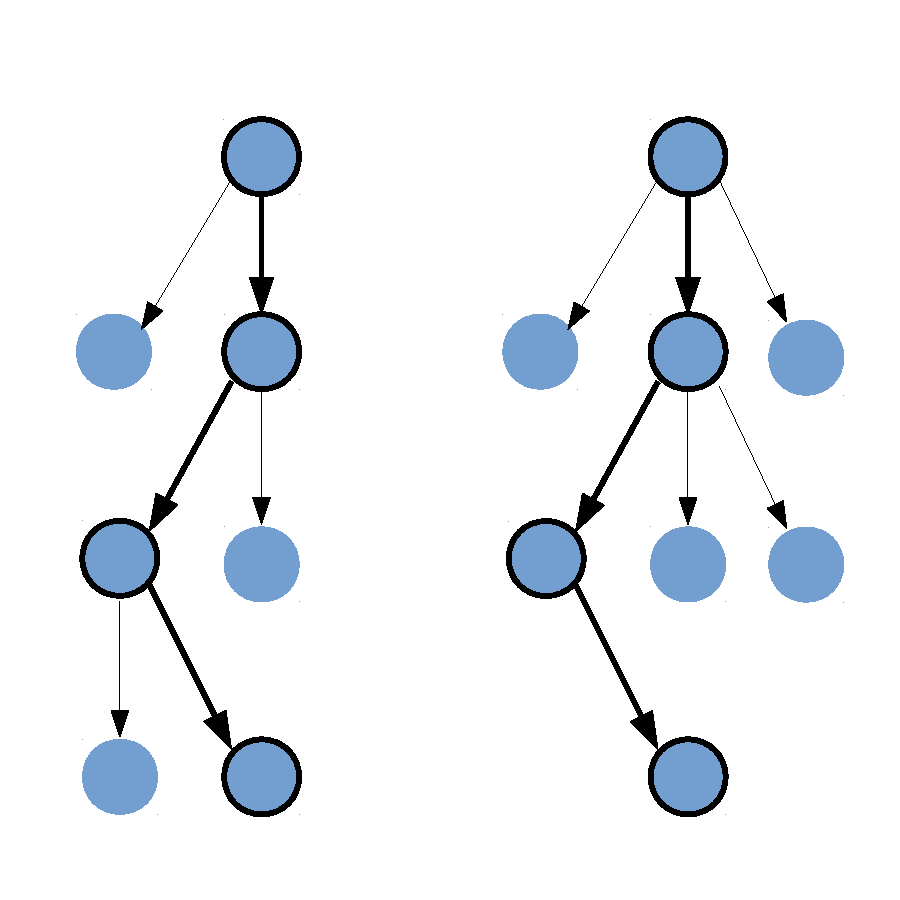
\includegraphics[width=0.5\textwidth]{fork_fig.pdf}
				\caption{Though local copies of the blockchain differ,
					they ``eventually'' agree identically on the
					\textbf{global chain}}
			\end{figure}
		\end{column}

		\begin{column}{0.5\textwidth}
			\begin{itemize}
				\item The Bitcoin blockchain is the prototypical blockchain
				\item Distinct nodes in the Bitcoin network each hold their
					own copy of the \textit{entire} history of transactions
				\item Each block must reference a pre-existing block using a hash function
				\item Guarantees \textbf{proof of work}
				\item Bitcoin ensures (in probability) that local copies of the blockchain
					will eventually agree on which chain is \textbf{global}
			\end{itemize}
		\end{column}
	\end{columns}
\end{frame}

\begin{frame}
	\frametitle{Three networks evolving simultaneously}

	\begin{columns}
		\begin{column}{0.3\textwidth}
			\centering
			\textbf{SPAN}
			\begin{figure}
				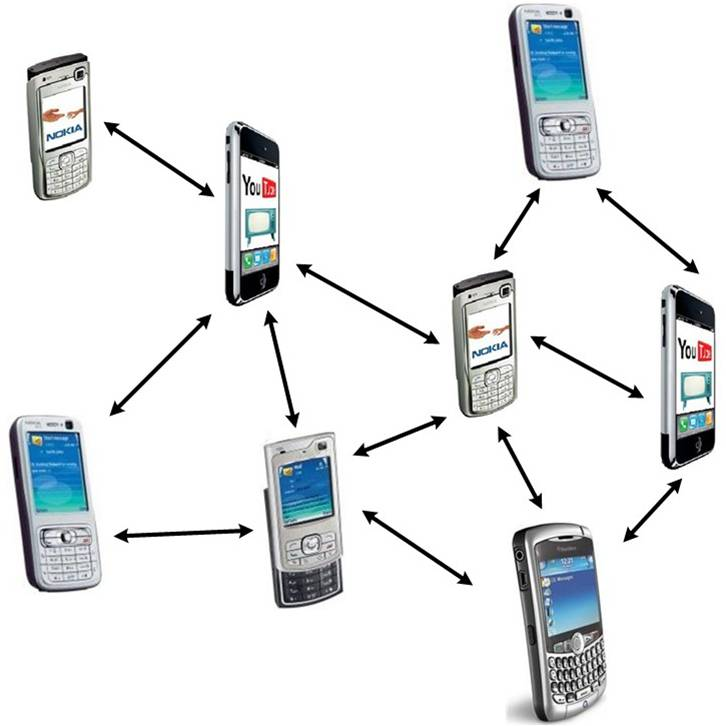
\includegraphics[width=\textwidth]{span.jpg}
			\end{figure}
			\begin{scriptsize}
				\begin{itemize}
					\item Nodes enter/leave the network all the time
					\item Network essentially always fragmented
				\end{itemize}
			\end{scriptsize}
		\end{column}

		\vrule{}

		\begin{column}{0.3\textwidth}
			\centering
			\textbf{Local Blockchain \\ (for each node)}
			\begin{figure}
				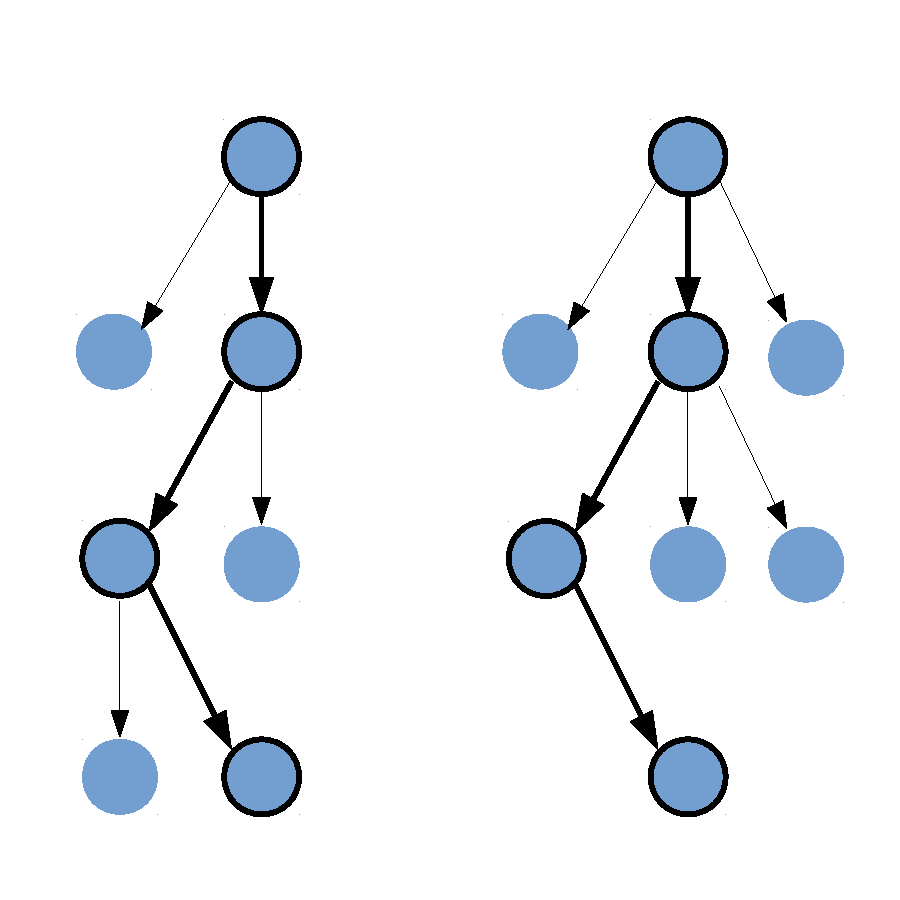
\includegraphics[width=\textwidth]{fork_fig.pdf}
			\end{figure}
			\begin{scriptsize}
				\begin{itemize}
					\item Unique tree of blocks for each node
					\item Tree growth contingent on the ``checkins'' to which
						node is privy
				\end{itemize}
			\end{scriptsize}
		\end{column}

		\vrule{}

		\begin{column}{0.4\textwidth}
			\centering
			\textbf{Global Blockchain...?}
			\begin{scriptsize}
				\begin{itemize}
					\item Conventionally, induced as the set-theoretic
						intersection of all local blockchains...
					\item But we are no longer guaranteed that this
						intersection would be a growing tree
					\item Per Nakamoto: For each node,
						there exists a neighborhood of nodes for which
						a global chain (at least among these neighbors) is
						well-defined
					\item \textbf{Hope:} Each such \textbf{neighborhood chain}
						corresponds to interaction of nodes within
						geographic proximity over some appreciable timescale
				\end{itemize}
			\end{scriptsize}
		\end{column}
	\end{columns}
\end{frame}

\begin{frame}
	\frametitle{What we accomplished:}

	\begin{enumerate}
		\item \textbf{Write protocol that allows for the formation of
			blockchains in the manner described}
			\begin{itemize}
				\item Must be robust to first-order
					adversarial behavior
			\end{itemize}
		\item \textbf{Simultaneously simulate SPAN and local blockchains
			under this protocol}
			\begin{itemize}
				\item Simulate evolution of SPAN using \textbf{random
					geometric graphs}
				\item Run blockchain protocol as the SPAN evolves to
					create varying local chains
				\item Tune parameters so that protocol creates
				neighborhood chains corresponding to geographic
				locales
			\end{itemize}
	\end{enumerate}
\end{frame}

\begin{frame}
	\frametitle{1) The Protocol}
	\begin{columns}
		\begin{column}{0.3\textwidth}
			\hfil
			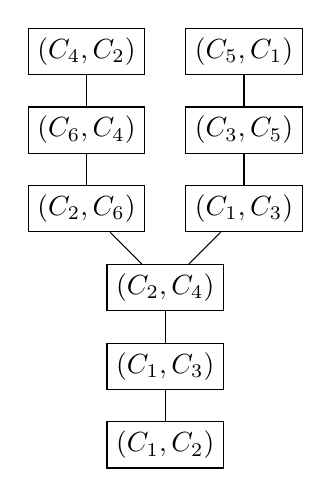
\begin{tikzpicture}[
					every node/.style = {
						shape = rectangle,
						draw,
						minimum width = 1cm,
						minimum height = 0.5cm,
					},
			]
				\draw (0, 0) node (a1) [rectangle] {$(C_1, C_2)$};
				\draw (0, 1) node (a2) [rectangle] {$(C_1, C_3)$};
				\draw (0, 2) node (a3) [rectangle] {$(C_2, C_4)$};
				\draw (1, 3) node (b4) [rectangle] {$(C_1, C_3)$};
				\draw (1, 4) node (b5) [rectangle] {$(C_3, C_5)$};
				\draw (1, 5) node (b6) [rectangle] {$(C_5, C_1)$};
				\draw (-1, 3) node (c4) [rectangle] {$(C_2, C_6)$};
				\draw (-1, 4) node (c5) [rectangle] {$(C_6, C_4)$};
				\draw (-1, 5) node (c6) [rectangle] {$(C_4, C_2)$};

				\draw (a1) -- (a2);
				\draw (a2) -- (a3);
				\draw (a3) -- (b4);
				\draw (b4) -- (b5);
				\draw (b5) -- (b6);
				\draw (a3) -- (c4);
				\draw (c4) -- (c5);
				\draw (c5) -- (c6);
			\end{tikzpicture}
		\end{column}

		\begin{column}{0.7\textwidth}
			\begin{itemize}
				\item Cryptographic challenge: Tuple $(t_C, k_C)$
					\begin{itemize}
						\item $k_C$ is the public key of the creator
						\item $t_C$ is timestamp of the problem creation
					\end{itemize}
				\item Block: Tuple $B = (t_C, k_C, t_S, k_S, n, b)$
					\begin{itemize}
						\item $(t_C, t_S)$ is a cryptographic challenge
						\item $t_S$ is the timestamp of the solution
						\item $k_S$ is the public key of the solver
						\item $n$ is the solution nonce
						\item $b$ is a pointer to a previous block
					\end{itemize}
				\item Hashing: $H(B) < \tau$
				\item Nodes exchange cryptographic challenges
				\item Handshakes are recorded in the ledger
					in the form of blocks
			\end{itemize}
		\end{column}
	\end{columns}

\end{frame}

\begin{frame}
	\frametitle{2) SPAN Simulator Package}

	\begin{columns}
		\begin{column}{0.3\textwidth}
			\centering
			\begin{figure}
				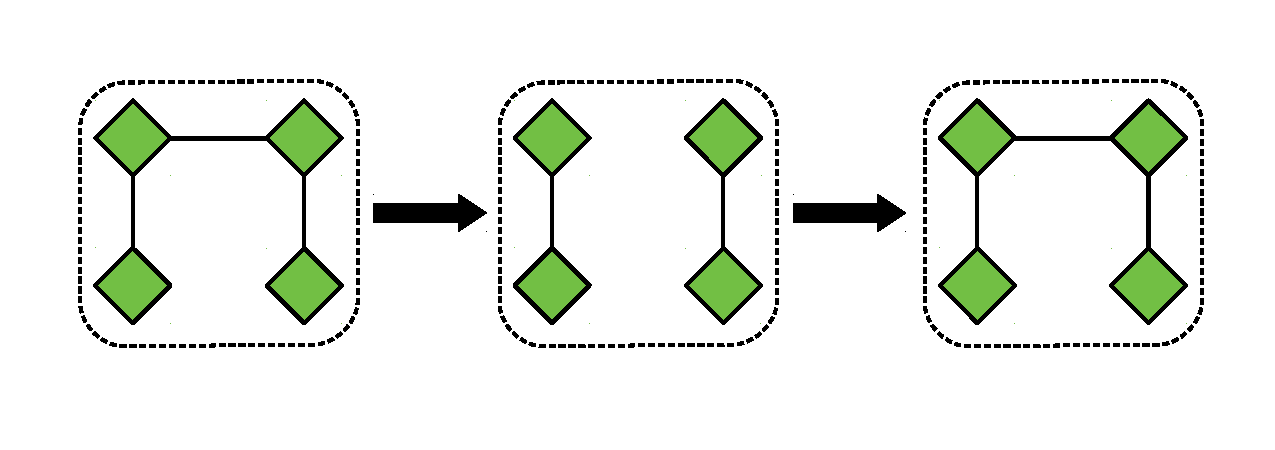
\includegraphics[width=\textwidth]{horseshoe.pdf}
				\caption{Progression of a SPAN topology over time}
			\end{figure}

			\vspace{-1cm}

			\begin{figure}
				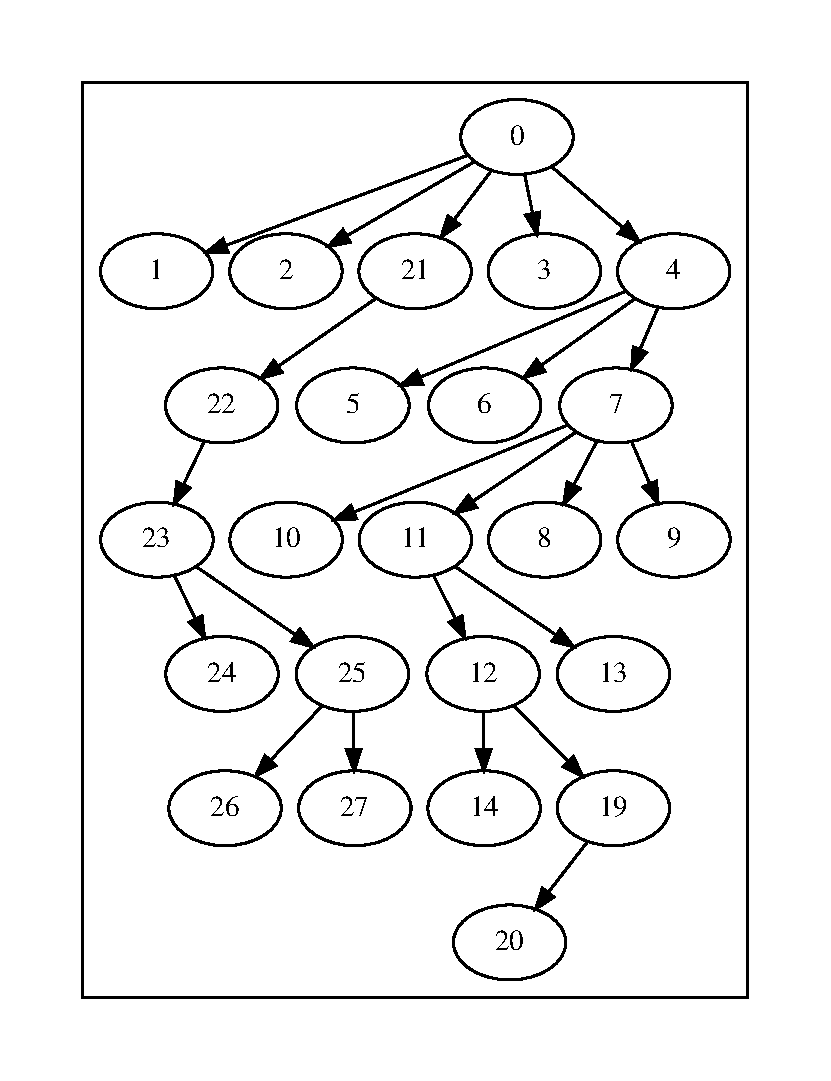
\includegraphics[width=\textwidth]{horseshoe_0.pdf}
				\caption{A local blockchain formed during the above
				progression}
			\end{figure}
		\end{column}

		\begin{column}{0.7\textwidth}
			\centering
			\begin{itemize}
				\item Written as a general platform for simulation
					of SPANs and blockchains distributed over
					SPANs
				\item SPAN Simulation
					\begin{itemize}
						\item Written to allow for static or dynamic
							topologies
						\item Accommodates various kinds of randomized
							SPAN evolution
					\end{itemize}
				\item Message passing per described protocol
				\item Local blockchain formation
				\item Visualization
					\begin{itemize}
						\item Captures and exports state information for
							each message-passing step and each change in
							SPAN topology
					\end{itemize}
			\end{itemize}
		\end{column}
	\end{columns}	
\end{frame}

\begin{frame}
	\frametitle{Future Work: Quantifying Neighborhood Chains}

	\begin{columns}
		\begin{column}{0.5\textwidth}
			\centering
			\begin{figure}
				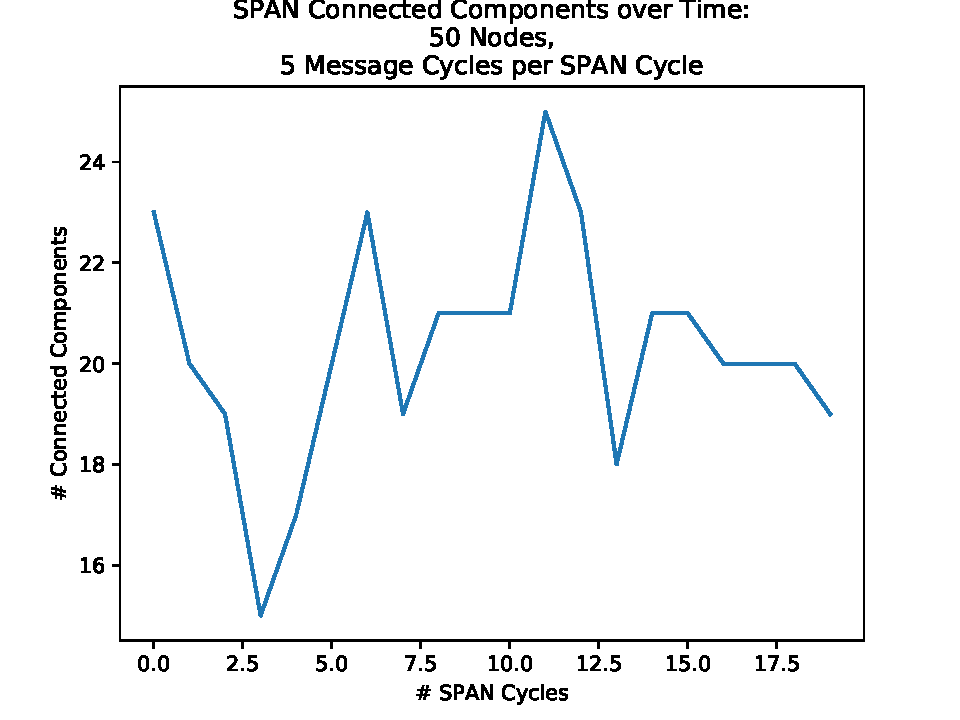
\includegraphics[width=\textwidth]{adj_mat.pdf}
				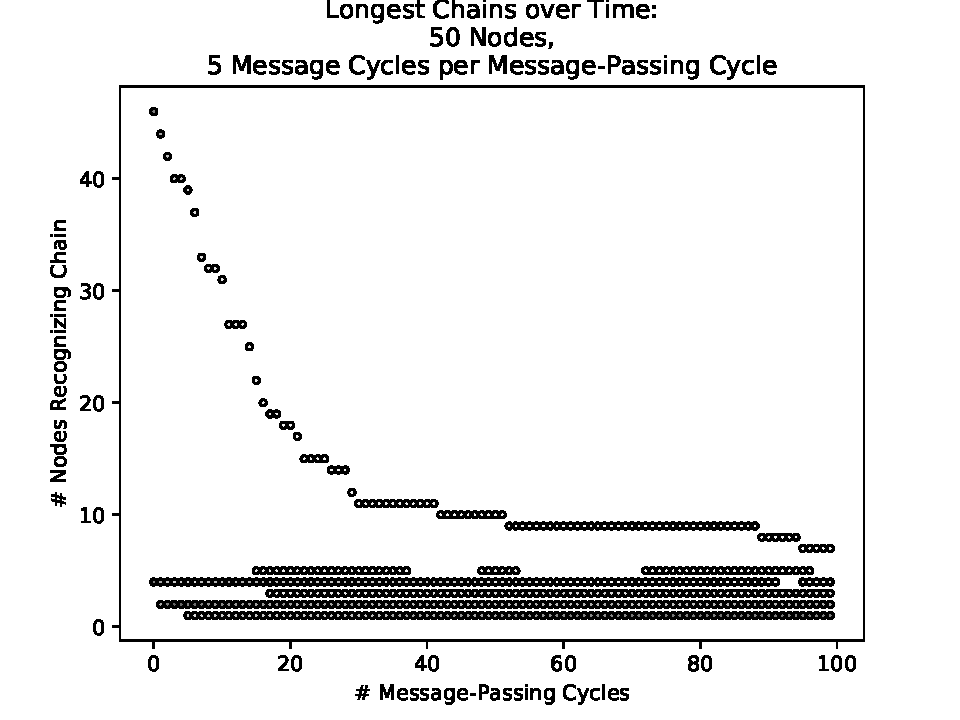
\includegraphics[width=\textwidth]{longest_chain_hist.pdf}
			\end{figure}
		\end{column}

		\begin{column}{0.5\textwidth}
			\begin{itemize}
				\item Uncharted Territory: measuring degree to
					which global blockchain is
					undefined is uncharted territory
					\begin{itemize}
						\item Try doing this with neighborhood blockchains
						\item Identify each \textbf{longest chain} in
							local blockchain with its \textbf{leaf}
						\item Calculate percentage of nodes for which leaf
							appears as \textbf{maximal node} of a longest chain
					\end{itemize}
				\item Look at distribution of neighborhood chains
					as function of number of SPAN connected components
			\end{itemize}
		\end{column}
	\end{columns}
\end{frame}

\end{document}
